\section{Ordinary binary and Koblitz research}\label{sec:binary}

\subsection{What the Koblitz structure buys}

The Frobenius-invariant base implementation checks invariance point by
point, folds columns into Frobenius orbits and carries the corresponding
known $\lambda^k$ weights into relations. Small-field records report
roughly degree-$n$ savings in relation bookkeeping and degree-$n^2$
savings in linear algebra, consistent with the known invariant-base
method. Rho also uses the available signed-Frobenius quotient, whose
idealised improvement is of square-root orbit size. Comparing IC to rho
without that available quotient would credit IC with a symmetry the
reference was unnecessarily denied.\src{KOBLITZ}\cite{ggmp2020}

The progression from invariant subspaces to divisor bases, SAT-optimised
bases, rank-guided constructions and compact signed-Frobenius orbit bases
is an important implementation record. The compact base stores orbit
representatives and their known scalar weights rather than an entire
quadratic pair table. It trades memory and rank-generation behaviour
against online probes. It is the closest IC family to rho in several
recorded small-curve comparisons, but its advantage relative to another
IC construction is not a claim that it beats matched rho.\src{COMPACT}
\src{FRONTIER}

\subsection{Correctness improvements underneath the speedups}

The September development record includes a consequential root-kernel
repair. A previous combined-inversion implementation treated equal or
zero abscissae as rootless, although the specialised $S_3$ equation becomes
linear or a square equation in those cases. Exceptional scans consequently
installed false nogoods. The repaired kernel handles those degeneracies;
its source includes exhaustive root-set comparison for all 16,384
abscissa pairs over $\F_{2^7}$ and larger-field checks through degree 53.
The historical degree-53 SAT example retains the same planted relation and
3,631 conflicts while removing 39,856 false nogoods. Pre-repair certificate
schemas fail closed rather than being silently accepted.\src{KOBLITZ}
\src{KOBLITZ-ARITH}

The same record repairs a nonmonic-pivot rank-tracker error. These are
correctness gains even when a headline solve time does not change.
Word arithmetic, batched inversions and cofactor projections then reduce
allocation and field-operation costs. The recorded Itoh--Tsujii schedule
uses seven rather than fifty-one multiplications at degree 53, but its
microbenchmark difference is below that host's timing noise. Lexicographic
SAT symmetry breaking increased conflicts and was left disabled. Such
rejected and inconclusive changes belong beside successful optimisations.
The source reads in this review are not fresh Rust test executions.
\src{KOBLITZ}\src{S3-COST}

\subsection{Production improvements that survive a narrow reading}

Free relations harvested from the root table are a concrete example of a
mechanism that is useful but smaller than first hoped. A degree-61 census
with 600 columns finds 147 nontrivial collisions but only 49 independent
relations against 599 required. The original predicted yield was about
60 times too high. That defeats the proposed large rank shortcut at the
tested construction; it does not make every free relation worthless.
\src{EQUAL}

The later production comparison tunes the baseline and candidate rather
than comparing a tuned candidate to an untuned incumbent. Its held-out
candidate/incumbent counted ratio is 0.960, with interval
[0.946,0.976], over 360 verified runs. The feature is on by default with
a switch restoring the previous path, and the study records exact A/A
behaviour. At the same fixed $K$, the degree-41 and degree-53 intervals
include one; degree 61's 0.962 remains the clean same-$K$ effect. The
earlier pooled 0.957 result is annotated not to be reused as the tuned
claim.\src{ROUND1}\src{ROUND2}

This is measurable, modest production engineering. It also illustrates
why ``a major lead did not produce its hoped-for yield'' and ``a useful
constant-factor improvement landed'' can both be true.

\subsection{N83: an exact cold-process example}

The five-point N83 holdout compares nearby compact-base sizes under a
frozen winner rule and Tier-1 cloud conditions. Its curve is
\texttt{icv1-f2m83-t6151469093347-9eba6cd5}, with model
$y^2+xy=x^3+x^2+1$, prime subgroup order
$r=8,569,786,107,849,059$ and cofactor 1,128,547,018.
The subgroup has about 53 bits; ``N83'' is the field degree, not an
83-bit prime-order subgroup.\src{N83}\src{N83-ROWS}

It is also a different model from the exact E0 degree-83 fidelity gate
in the repository contract: $y^2+xy=x^3+1$, subgroup order
2,417,851,639,230,796,216,685,689 and cofactor four. That E0 subgroup
has about 81 bits. The E1 holdout above is useful evidence for its own
workload, but matching field degree alone does not discharge that exact
E0/ECC2K-130 fidelity obligation.\src{C-RULES}

\begin{table}[htbp]\small
\caption{Recorded five-point cold-process means. The baseline's two
A/A child times are averaged per point before the panel mean. This is
a configuration comparison within IC, not a comparison of matched cold
IC and rho. Source: \src{N83-ROWS}.}
\begin{tabular}{@{}lrrrr@{}}\toprule
Columns & Usable points & Cold seconds & Setup seconds & Rank seconds \\\midrule
1,104 & 183,264 & 120.227 & 48.728 & 71.320 \\
1,108 & 183,928 & 121.296 & 48.955 & 72.171 \\
1,120 & 185,920 & 119.826 & 50.081 & 69.525 \\
1,152 & 191,232 & 122.471 & 53.067 & 69.255 \\\bottomrule
\end{tabular}
\end{table}

The 1,120-column arm saves 2.645 seconds over 1,152 columns, with paired
95\% interval [2.085,3.205] seconds. The 1,104-column arm saves 2.244
seconds, interval [1.980,2.508]. But the observed 0.401-second advantage
of 1,120 over 1,104 columns has interval [$-0.236$,1.038], so the frozen
selection remains \texttt{BOUNDED\_UNKNOWN} with no selected candidate
identifier. All 25 IC arms and five rho arms have recorded independent
replay, and the study retains five passing baseline A/A gates.

\begin{figure}[htbp]
\centering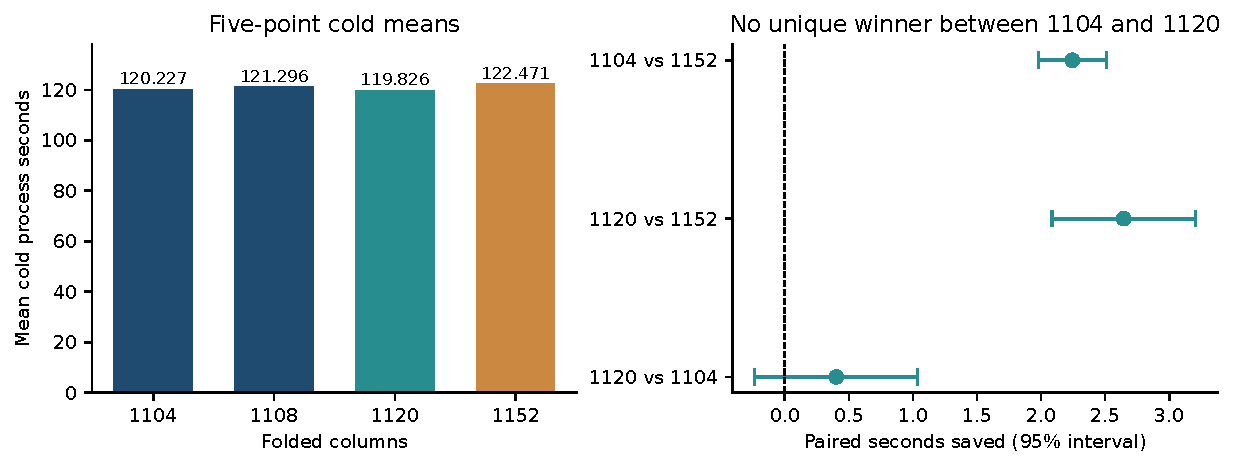
\includegraphics[width=\linewidth]{figures/n83.pdf}
\caption{A verified, held-out IC configuration improvement without an
overstated winner. Left: recorded cold-process means. Right: paired
seconds saved over the 1,152-column baseline, with the recorded 95\%
intervals; the final row compares the two leading candidates and includes
zero. Five public workloads, Tier-1 cloud instance. Source: \src{N83-ROWS}.}
\end{figure}

The setup/rank split identifies the next bottleneck more usefully than a
headline online ratio. Rank generation accounts for about 69--72 seconds
in these means, while target online work is a fraction of a second.
Reducing retained-state query latency alone cannot remove the cold rank
cost. Different base sizes also move the two phases in different
directions, which is why the winner rule should remain attached.

\subsection{Online ladders and the preprocessing control}

The historical ladder reaches degrees 53, 61, 71, 73 and 83, including
128-bit field packing beyond degree 64. The degree-61 two-host panel
records a 13.94 online rho/IC median ratio with interval [9.81,19.13]
on 64 fresh workloads, with roughly 28 seconds of setup excluded. These
are actual observations under that retained-preparation question.
\src{PRIOR}\src{COMPACT}

The equal-advice audit changes their interpretation. At degrees 41, 53
and 61, preprocessing rho uses the same or less retained advice and is
reported 53--317 times faster online by ratios of means; setup costs
are separately shown and are not matched in every such row. Some
controls fail their original prediction, and the host is contended.
Consequently the retrospective preserves the measurements, their
control caveats and their setup boundary, rather than treating them as
a universal dominance theorem.\src{EQUAL}

At degree 83, a later study runs time-matched and RSS-matched
Bernstein--Lange controls on 16 public points. Its K3300 time-matched
median IC/preprocessed-rho ratio is 3.74, interval [2.65,11.05]; its
RSS-matched ratio is 40.61, interval [24.27,71.72]. Its K600 comparisons
are larger. Under that protocol, neither original ``IC beats rho''
online interpretation survives matched preprocessing. The study also
states that no operation-count ranking is admitted: one band's order
flips, while another arm omits root-call emission.\src{EQUAL83}

The equal-bytes, single-process-group wide experiment at degrees 73
and 83 is nevertheless a distinct open requirement. Its instrument is
built and checked, but the frozen wide session is explicitly not run.
Time-matched and RSS-matched experiments should not be relabelled as
that missing experiment.\src{WIDE}

\subsection{Ordinary binary oracles and solving degree}

The ordinary-binary programme includes XOR-aware SAT, Semaev systems,
matrix F4, inherited F4, pair-and-solve oracles, meet-in-the-middle tables
and root finding. A binary MITM ladder reaches $\ell=12$, where the
recorded table has about 8.09 million sums and occupies about 259 MB.
The maximum counted query work is 16,092 point additions against about
8.39 million quartic solves in the comparator; witnesses and negative
answers are cross-checked on the panel. The table is target-independent
setup and is charged as such. The large query improvement is not an
end-to-end exponent improvement.\src{TIMELINE}

The degree-closure studies make another important distinction: plain
XL degree, first-fall degree, closure refutation degree and the cost of a
full Gröbner solve are not interchangeable. Full closure can refute a
system several degrees below an XL-only diagnostic. In the recorded
scale studies, two explanations survive the tested cells: a rise near
$\ell=7$, or a rise when $m\ell\ge21$. The $m=4,\ell=6$ cell separates
them and remains unmeasured at the required boundary. The sparse closure
is an independent correctness check on smaller instances, but is too
slow to resolve that boundary in the recorded experiment.\src{DREG}

For ECC2K-130, degree-five extrapolations are therefore optimistic
scenarios rather than measured cryptographic-scale solvers. The
reported $2^{71.13}$ row is in unconverted column-touch units, whereas
the $2^{60.81}$ rho figure is in group operations. A displayed
``10.32-bit gap'' is an arithmetic comparison of those model entries,
not a calibrated attack-cost ratio. Neither a memory failure nor the
absence of a favourable row proves a general lower bound on binary IC.
\src{DREG}\src{LEADS18}
